\chapter{Time Projection Chamber}
\label{sec:tpc}
	\textcolor{red}{Using (2010 -- a little old) https://cds.cern.ch/record/1302071/files/CERN-PH-EP-2010-047.pdf}
	
	A~\acf{TPC} is a~type of gaseous detector that uses the~drift in an~electric field of free charges (electrons and cations) produced by an~ionizing particle to reconstruct its 3D~trajectory. When placed inside a~magnetic field, the~momentum of the~incident particle can be inferred from the~curvature of its trajectory. Particle identification is also possible using the~ionization energy loss inside the~\ac{TPC}.
	
	The original \ac{TPC} used in the~PEP-4 experiment at SLAC was a $2\times2$~m cylinder with a~central cathode that produced a~strong electric field, making the~ionization electrons drift towards one of the bases. The~readout consisted of \ac{MWPC}s, where electrons are accelerated towards the~anode wires enough to further ionize the~gas and cause an avalanche. \textcolor{red}{Figure?}
	
	When a~charged particle crosses the~volume of a~\ac{TPC}, it loses energy by excitation and ionization of the detector gas. Most ionizing collision produce a~single ionization electron, sometimes a~few secondary electrons are produced close to the~collision vertex. In rare cases, the~ionization electron has energy large enough to create a measurable track, such an~electron is called a~$\delta$\nobreakdash-electron.
	
	\textcolor{red}{CERES/NA45 -- very inhomogeneous magnetic field}
	
	\section{Charge transport in gases}
		\subsection{Drift}
			The~produced ionization electrons are accelerated towards the~readout by the~electric field inside the~chamber. At the same time, they lose speed by colliding with the~gas particles, quickly reaching a~constant (for a~given field $\mathbf{E}, \mathbf{B}$) mean drift velocity. The~electrons might be absorbed by electronegative impurities, such as halides and oxygen.
			
			In many gases (called "hot", e.g., Ar or CH$_4$), the~drift velocity is much greater than that of their thermal motion thanks to a~high proportion of elastic collisions. On the other hand, "cold" gases like CO$_2$ have a higher proportion of inelastic collisions (e.g., thanks to the~excitation of rotational and vibrational states) and therefore much lower drift velocity.
			
			The cations produced by the~ionization lose a significant portion of their energy during each collision thanks to their large mass. This makes their drift velocity much smaller and their energy is close to thermal. Since their momentum isn't randomized to such extent during collisions, their diffusion is smaller.
			
			The drift is also influenced by the~magnetic field, Langevin derived a~good approximation for the~drift velocity vector:
				\begin{equation}
					\mathbf{v}_\text{d} = \left(\frac{\mathbf{E}}{\norm{\mathbf{E}}} + \omega\tau\frac{\mathbf{E}\times\mathbf{B}}{\norm{\mathbf{E}}\norm{\mathbf{B}}} + \omega^2\tau^2\frac{\mathbf{E}\cdot\mathbf{B}}{\norm{\mathbf{E}}\norm{\mathbf{B}}}\cdot \frac{\mathbf{B}}{\norm{\mathbf{B}}}\right) \frac{q\tau}{m(1+\omega^2\tau^2)}\norm{\mathbf{E}},
				\end{equation}
			where $q$ is the~charge of the particle, $m$ is its mass, $\tau$ is the mean time between collisions and $\omega = \frac{q}{m}\norm{\mathbf{B}}$. In a~standard \ac{TPC}, $\mathbf{E}$ is nearly parallel to $\mathbf{B}$ and only small corrections are needed. The~ion drift is only negligibly influenced by the~magnetic field ($\omega\tau\sim10^{-4}$ is small). \textcolor{red}{Lorentz angle for orthogonal fields $\tan\psi = -\omega\tau$ (deviation from electric field) -- maybe mention in the OFTPC section.}
		\subsection{Diffusion}
			Due to random collisions a~point-like cloud of electrons or ions will show a~Gaussian density distribution at time $t$ due to the drift in electric field $\mathbf{E} = (0,0,E_z)$:
				\begin{equation}
					\rho(x,y,z,t) = (4\pi Dt)^{-\frac{3}{2}} \exp\left(-\frac{x^2+y^2+(z-v_dt)^2}{4Dt}\right),
				\end{equation}
			where $D$ is the diffusion coefficient given by
				\begin{equation}
					D = \frac{\lambda^2}{3\tau} = \frac{\lambda v_\text{d}}{3} = \frac{v_\text{d}^2\tau}{3} = \frac{2\varepsilon\tau}{3m},
				\end{equation}
			where $\lambda$ is the mean free path and $\varepsilon$ the mean energy. The lateral diffusion width $\sigma_x$ after a drift distance $L$ can be expressed as
				\begin{equation}
					\sigma_x^2 = 2Dt = \frac{4\varepsilon L}{3qE}.
				\end{equation}
			The minimal diffusion width is given by lowest possible (thermal) energy of the~particles $\varepsilon_\text{th} = \frac{3}{2}kT$:
				\begin{equation}
					\sigma_{x, \,\text{min}}^2 = \frac{2kTL}{qE}.
				\end{equation}
			For electrons in "cold gases" (e.g., Ar/CO$_2$ mixture), the diffusion approaches this limit up to a~certain field intensity ($\sim 100~\text{V}/\text{cm}$ at 1~atm pressure). \textcolor{red}{For us 0.45~mm, quite close to the actual diffusion 0.5-0.7~mm.} In reality, the~transversal diffusion of electrons can be significantly different from their longitudinal diffusion, simulations are necessary to achieve a~precise calculation.
			
			In most \ac{TPC}s, the~transversal (but not the~longitudinal) diffusion is reduced by the~magnetic field (parallel to electric):
				\begin{equation}
					\frac{D_\text{T}(B)}{D_\text{T}(0)} = \frac{1}{C+\omega^2\tau_2^2},
				\end{equation}
			where $C$ and $\tau_2$ are parameters dependent on the~gas.
	
	\section{Readout}
		\subsection{Multi-Wire Proportional Chamber}
			In most \textcolor{red}{(2010 -- almost all)} \ac{TPC}s operated in experiments \acf{MWPC} was used for the~readout. The electrons enter the chamber through a~cathode grid and get accelerated in the~strong electric field towards the~thin anode wires and create a~Townsend avalanche, multiplying the~signal. \textcolor{red}{Alternating with field wires?} The~trajectory can be reconstructed using pulses from each separate wire. Segmented cathode is also often used for the readout of produced cations. \textcolor{red}{Gating grid (reduction of space charge effect, blocking backflow of ions?, closed for electrons B=0, $\Delta V$, static mode (loss of 25\% el.) x opening on trigger)? (gas amplification $>10000$ required for good SNR, 100-200~ns shaping time), figure?}
			
		\subsection{Gas Electron Multiplier}
			The~\acf{GEM} is a~thin metal\nobreakdash-coated polymer sheet with a~high density of small holes. The amplification is achieved by applying voltage on the~metal layers, creating a strong electric field inside the~holes and causing avalanches. Double or triple stack of \ac{GEM}s is usually used to create a~sufficient gain. From the last foil, the~electrons drift to a~segmented anode where the~signal is read. The~backflow of cations is reduced compared to \ac{MWPC}. \textcolor{red}{Picture of Garfield simulation. Parameters?}
		
		\subsection{Micromegas}
			In a~\ac{Micromegas} electrons pass through a~fine mesh (made out of very thin wires) into the~narrow amplification gap where they are multiplied in the~high field and read as signal on the~segmented anode. Very high field (30-80 kV/cm$^2$) is necessary to achieve sufficient gain. Cation backflow is heavily suppressed by the~mesh.
			
		\subsection{Parallel Plate Chamber}
			\textcolor{red}{...}
			
			
	
	\section{Orthogonal Fields TPC at IEAP CTU}
	\label{sec:oftpc}
		\textcolor{red}{Short description of our detector. Why we use an~atypic TPC (benefits, complications). Gas mixture used in the~detector (70/30) and its effect.}
	
		\subsection{Coordinate Systems}
		\label{sec:coor}
			In order to describe events in our detector, we use three distinct spaces: the~detector space $\mathcal{D}$, the~readout space $\mathcal{R}$ and the~pad space $\mathcal{P}$. Each space is later used to represent ionization electrons at different stages of the~detection process: their creation in the gas, their final position when hitting the readout plane, and finally their representation in the discrete pad space.
		
			\subsubsection{Detector Space}
				The~detector space $\mathcal{D}$ represents the~physical space of our detector. We describe it using Cartesian coordinates $(x,y,z)$. The~$z$-axis is the~detector's axis of symmetry, with its negative direction aligned with the~proton beam. The~origin $(0,0,0)$ is located at the~center of the~irradiated target. The~positive $x$\nobreakdash-axis passes through the~center of one the~\ac{OFTPC}s along the~intersection of its two planes of symmetry. The~$y$\nobreakdash-axis is then chosen to maintain a~right-handed coordinate system.
				
				Since the~detector has a~hexagonal symmetry, we use only one of its sectors in this work -- the~first sector $\mathcal{D}_1 \subset \mathcal{D}$ which is defined by the~condition:
					\begin{equation}
						(x,y,z) \in \mathcal{D}_1 \Leftrightarrow |y| \leq x\tan \frac{\pi}{6}.
					\end{equation}
				Simulations in this sector can be applied to all sectors by rotating the coordinates accordingly. The~volume of the~\ac{OFTPC} in this sector, which has the~shape of a~trapezoidal prism, has these boundaries:
					\begin{linenomath}
						\begin{align}
							x \in [x_\text{min},x_\text{max}] &= [6.51, 14.61] \;\text{cm},\\
							z \in [z_\text{min},z_\text{max}] &= [-8,8] \;\text{cm},\\
							y_\text{max}(x_\text{min}) = -y_\text{min}(x_\text{min}) &=  2.75\;\text{cm},\\
							y_\text{max}(x_\text{max}) = -y_\text{min}(x_\text{max}) &=  7.45\;\text{cm},
						\end{align}
					\end{linenomath}
				where $y_\text{max}(x)$ is the~maximal value of the~$y$-coordinate for a~given $x$. The~readout is located at $z = 8$~cm; for some purposes, we also define the distance to the~readout $d_r = 8\;\text{cm}-z$ as an~alternative to the~$z$-coordinate. \textcolor{red}{Keeping this paragraph as it is because the~\ac{OFTPC} volume is distinct from the~first sector and some parts of this thesis use the~space beyond this volume.}
			
			\subsubsection{Readout Space}
				The~readout space $\mathcal{R}$ represents the~drift time and final positions of ionization electrons as measured by an~ideal continuous readout. We describe it using coordinates $(x',y',t)$, where $x'$ and $y'$ correspond to the~detector coordinates at the readout plane ($z = 8$~cm). \textcolor{red}{Currently not entirely sure how to put this into a~figure since only $x'$ and $y'$ correspond to the~detector coordinates. The drift time~$t$ is approximately proportional to~$d_r$.}
			
			\subsubsection{Pad Space}
				The~pad space $\mathcal{P}$ represents the~time bin and pad number of ionization electrons as measured by an~ideal discrete readout. \textcolor{red}{It is not really a~subspace of $\mathcal{R}$ but there is a mapping from $\mathcal{R}$ to $\mathcal{P}$. It is a discretization of a~part of $\mathcal{R}$, the mapping can be adjusted depending on the~simulation. If we assume uniform electric field there will be gaps, we don't use gaps in the reconstruction since the~electrons should be pulled towards the~pads.}
				
				The~readout of the~\ac{OFTPC} will consist (\textcolor{red}{is the design final?}) of 128~rectangular pads arranged in a~staggered pattern (\textcolor{red}{add image where all the parameters are marked}). Most of the~pads are $0.6 \times 0.9$~cm, only pads 102 and 124 are $0.6 \times 0.6$~cm, pad 127 is $0.6 \times 0.509$~cm. The~distance of neighboring pads is 0.08~cm, staggering offset is 0.3946~cm.
			
				\begin{figure}[H]
					\centering
					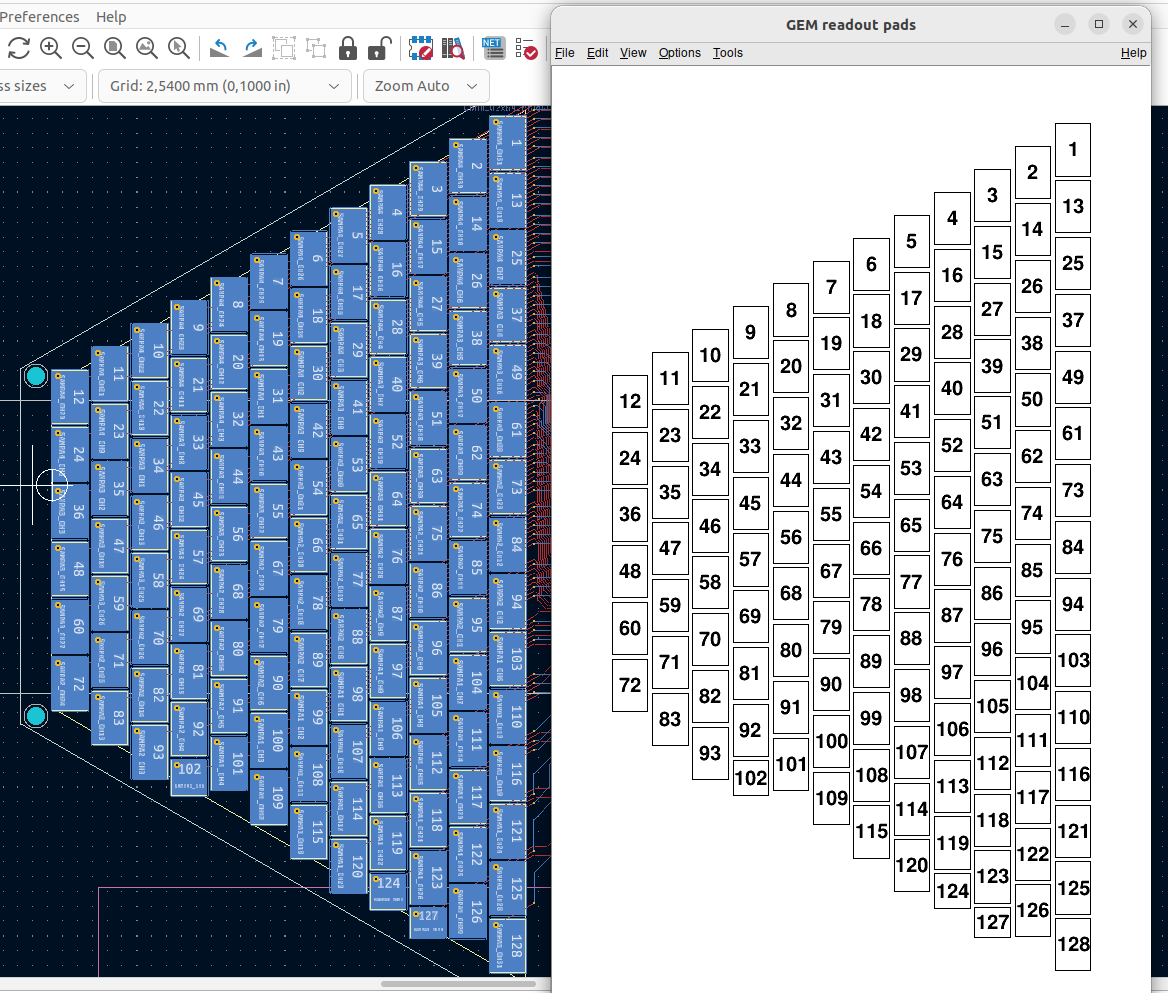
\includegraphics[width=0.8\textwidth]{padlayout.png}
					\caption{Pad layout of the~TPC. \textcolor{red}{Swap for better image.}}
					\label{fig:padlayout}
				\end{figure}
		
		\subsection{Magnetic Field Simulation}
		\label{sec:mag}
			\textcolor{red}{Magnetic field simulations in Maxwell (citation). Some figures. When working with the~magnetic field outside the~regular grid, we use trilinear interpolation.}
		
			\subsubsection{Trilinear Interpolation}
			\label{sec:trilin}
				Trilinear interpolation is a~3D generalization of linear interpolation. It can be used to interpolate a~function whose values are known on a~regular grid with rectangular prism cells. We use this simple method for interpolating the~magnetic field, and it is later used in Section~\ref{sec:grad} to interpolate the~Ionization Electron Map, a~key component of our track reconstruction algorithm. In both cases, we use a~regular cubic grid (\textcolor{red}{apparently it is also called a~Cartesian grid}).
				
				\textcolor{red}{Could put a~paragraph about linear interpolation here if it is not clear from the~equations below.}
				
				Let us consider a~cell of our regular grid (a~cube) with an~edge of length~$a$ containing the~point $\mathbf{C} = (x,y,z)$ where we want to interpolate a~function $f\!\!:~\!\!\mathbb{R}^3\,\to\,\mathbb{R}$. We know the~values of this function at the~vertices of the~cell $\mathbf{C}_{ijk} = (x_0+ia,y_0+ja,z_0+ka)$, where $i,j,k \in \{0,1\}$ are indices. We also define the~points $\mathbf{C}_{ij} = (x,y_0+ia,z_0+ja)$ and $\mathbf{C}_i=(x,y,z_0+ia)$. Then the~interpolated value $\widehat{f}(\mathbf{C})$ can be calculated as a~composition of three linear interpolations (see Figure~\ref{fig:trilin}):
					\begin{alignat}{3}
						\widehat{f}(\mathbf{C}_{ij}) &= (1-x_d)\,f(\mathbf{C}_{0ij}) \,&+&\,x_d\, f(\mathbf{C}_{1ij}),\\
						\widehat{f}(\mathbf{C}_{i}) &= (1-y_d)\,\widehat{f}(\mathbf{C}_{0i}) &+&\,y_d\, \widehat{f}(\mathbf{C}_{1i}),\\
						\widehat{f}(\mathbf{C}) &= (1-z_d)\,\widehat{f}(\mathbf{C}_0) &+&\,z_d\, \widehat{f}(\mathbf{C}_1),
					\end{alignat}
				where $x_d$, $y_d$, and $z_d$ are given as follows:
					\begin{equation}
						x_d = \frac{x-x_0}{a},~y_d = \frac{y-y_0}{a},~z_d = \frac{z-z_0}{a}.
					\end{equation}
				We can also write
					\begin{eqnarray}
						\widehat{f}(\mathbf{C}) = \sum_{i,j,k \in \{0,1\}} t_x^i t_y^j t_z^k f(\mathbf{C}_{ijk}),\\
						t_\alpha \stackrel{\text{def}}{=} \begin{pmatrix}t_\alpha^0\\ t_\alpha^1\end{pmatrix} = \begin{pmatrix}1-\alpha_d\\ \alpha_d\end{pmatrix},
					\end{eqnarray}
				where $\alpha \in \{x,y,z\}$ is an index. Furthermore, we can write $\widehat{f}(\mathbf{C})$ as a~polynomial:
					\begin{equation}
						\label{eq:trilinpoly}
						\widehat{f}(\mathbf{C}) = \sum_{\alpha,\beta,\gamma \in \{0,1\}}\sum^{\alpha}_{i=0}\sum^{\beta}_{j=0}\sum^{\gamma}_{k=0} 	(-1)^{(\alpha-i)+(\beta-j)+(\gamma-k)} f(\mathbf{C}_{ijk}) x_d^\alpha y_d^\beta z_d^\gamma.
					\end{equation}
				We take advantage of this form when generalizing trilinear interpolation to irregular grid in section~\ref{sec:interpol}.
					
					%\begin{equation}
					%	\widehat{f}(C) = (1-x_d) (1-y_d) (1-z_d) f(C_{000}) + (1-x_d) (1-y_d) z_d f(C_{001}) + (1-x_d) y_d (1-z_d) f(C_{010}) + (1-x_d) y_d z_d f(C_{011}) + x_d (1-y_d) (1-z_d) f(C_{100}) + x_d (1-y_d) z_d f(C_{101}) + x_d y_d (1-z_d) f(C_{110}) + x_d y_d z_d f(C_{111})
					%\end{equation}
				
				\begin{figure}[H]
					\centering
					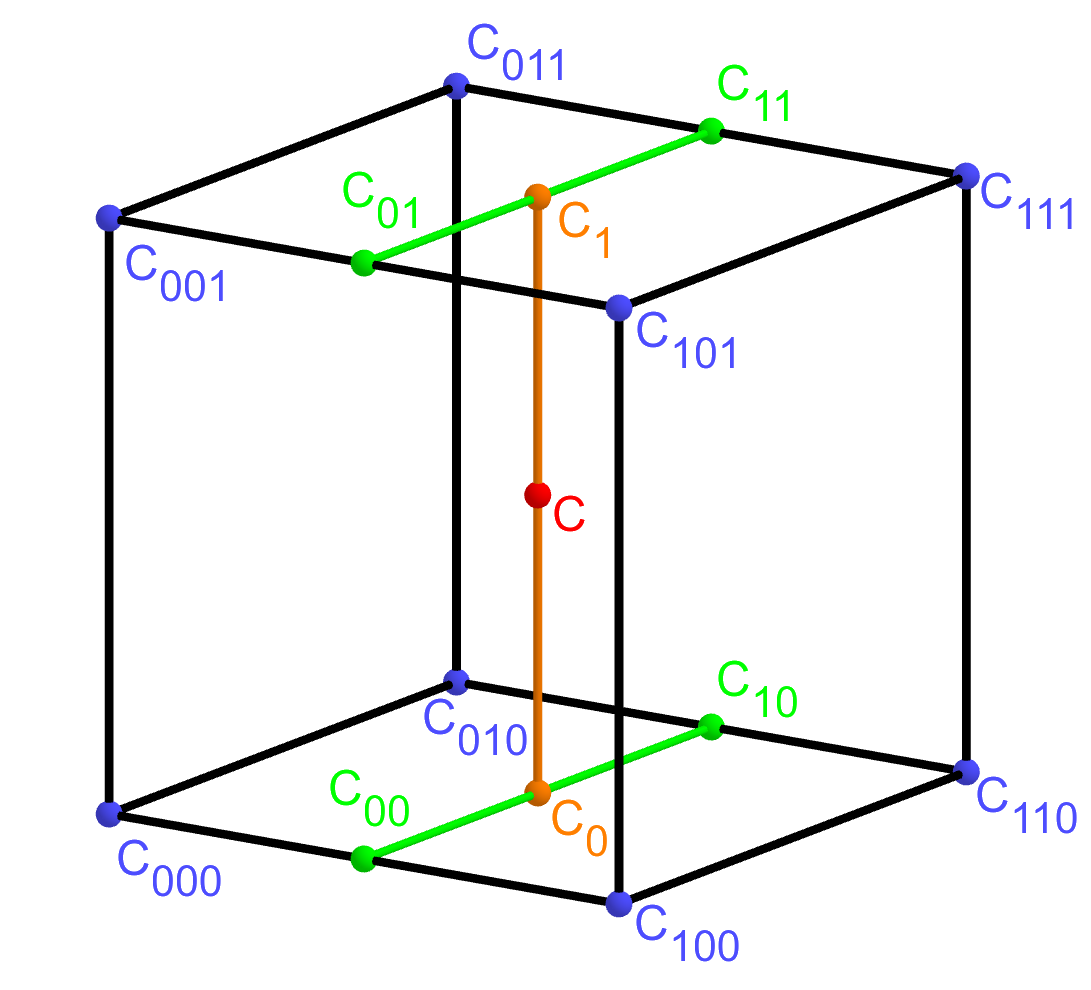
\includegraphics[width=0.5\textwidth]{trilinear.png}
					\caption{Visualization of trilinear interpolation as a~composition of linear interpolations. \textcolor{red}{Image drawn in GeoGebra and inspired by \href{https://commons.wikimedia.org/wiki/File:3D_interpolation2.svg}{a~similar image on Wikipedia} (which looks a~bit worse) -- is credit necessary?}}
					\label{fig:trilin}
				\end{figure}
				
				\textcolor{red}{Maybe a~citation here, although I am not sure it is necessary since it could be considered common knowledge. The~last two equations are my own. Maybe $x_0$, etc. should be explicitly described.}